% !Mode:: "TeX:UTF-8"
\documentclass[10pt,journal]{IEEEtran}
\usepackage{subfig}
\usepackage{graphicx}
\usepackage{amsmath}
\usepackage{algorithm}
\usepackage{algorithmic}
\usepackage{comment}
\usepackage{ctex}

\graphicspath{figures/}

\newtheorem{theorem}{Theorem}
\newtheorem{lemma}{Lemma}
\newtheorem{definition}{Definition}

\begin{document}
\title{基于OpenCL的网络演算数值计算库的改进算法}

\author{\IEEEauthorblockN{李宝亮}}
%\onecolumn
\maketitle

\begin{abstract}
网络演算已经取得了巨大的成功,但是以往针对网络演算的研究主要集中于对实际系统的分析和基于网络演算的建模,但是很少有研究现解决网络演算模型的快速计算问题。网络演算的数据计算库是网络演算应用的基本前提。尽管目前已经有一些面向分段线性伪周期函数的的网络演算数值计算库,但是这些库在处理阶梯函数时效率较低,特别是在进行卷积和闭包计算时。本文,我们提出一种基于区别覆盖的阶梯函数快速卷积计算方法,通过与Java计算库DISCO的比较,我们发现我们的方法在分析处理阶梯函数时效率大幅度提高。通过对该算法的分析,我们发现该算法的具有较高的可并行性,为了进一步提高计算性能,我们还基于OpenCL对这一算法进行了并行加速。实验结果表明,我们的计算方法较相应的串行方法性能提高10倍左右,较之前的基于java的算法相比,性能提高了近xxx倍。网络演算中卷积运行的快速计算,使得网络演算的应用更容易。
\end{abstract}
\begin{IEEEkeywords}
数值计算、并行算法、网络演算、延迟和积压界
\end{IEEEkeywords}

\section{Introduction}
网络演算的基本概念和应用情况。

网络演算的数值计算是网络演算面向实用的关键,没有一个高效的计算库,那么网络演算的性能分析则只能停留在理论层面,无法用于指导实际的网络分析和设计。网络演算是基于极小加代数得出的一种性能分析工具,由于其基于特殊的代数结构,而且卷积的计算和分析非常困难,因而使得其实际的分析和计算非常困难。目前很多的基于网络演算的研究都只考虑了采用网络演算来建模,但是在计算结果时则只能假设非常简单的到达和服务曲线模型,根本原因是网络演算的数据计算是非常复杂和困难的,即使是对非常简单的网络拓扑和模型,计算其端到端性能是也会涉及非常复杂的公式和推导,这使得计算结果变得非常困难。为了简化计算,在计算过程中通过会做一些简单,假设用一个较宽松但是非常简单的到达曲线(例如RB)和服务曲线(LR)来代替实际的网络服务曲线。又比较利用连续的到达曲线模型和服务曲线模型来简化实际的离散系统。这样做的直接后果是,所得到的结果较实际性能有更大的差异,原因是当采用近似的方法来简单系统时,会牺牲精度。另一方面,实际的通信系统(如计算机网络、ATM网络等)都是离散时间离散值的系统,因而采用离散模型来建模也更加直接,而且所得的结论也更好。另一方面,很多系统的分析过程中,必须采用离散的网络演算模型,例如基于实时网络演算的Flexray性能分析模型
\cite{Chokshi:2010:PAF:1774088.1774162,Hagiescu:2007:PAF:1278480.1278554},对于这类模型,如果采用连续服务模型会导致错误的结论;另外,还有一些情况,当采用离散时间模型时,也会非常方便和直观,一个典型的例子是基于实时网络演算的非抢占系统的性能分析\cite{4617308}。

但是,我们发现,当采用实时网络演算的工具箱来分析离散时间的到达和服务曲线模型时,是非常耗时的。以我们的论文中的例子,计算一组数据需要几十分钟的时间。通过对这类网络演算数据计算工具箱数值算法 的分析我们发现,这些工具箱都基于相同的算法\cite{Bouillard2008},这类算法面向分段线性伪周期函数类型的到达和服务曲线。所谓分段线性伪周期函数是指:。这类函数基本涵盖了网络演算理论中涉及的所有的模型。该算法假设所有的模型都是由无穷多的直线段组成的,直线段之间首尾相连,但是模型可以是不连续的,即可以存在瑕疵点。而分段线性伪周期函数函数都是由一些起始的非周期部分和后续的周期部分组成的,每一部分都是由若干个线段和瑕疵点组成。当整个函数中包含的线段数量(非周期部分+周期部分中一个周期内的线段数量)较少时,已有的算法便可以快速的给出结果,但是,当线段较多时,整个计算过程便会非常耗时。由于实际的系统都是离散的,因此,我们考虑一类非常普遍存在的情况:周期部分和非周期部分都很长,但是,每一部分中的线段数量也可以很多,但是,这些线段的斜率都为0,即整个的函数是阶梯函数。对于这类函数,本文,我们提出一类高效的计算方法,该方法的计算效率是原算法实现的数十倍。事实上,自然界的大部分模型都可以规约到这一类模型,因为通信系统都是离散时间系统。因而,我们的算法对网络演算的应用是非常重要的。

本文余下部分的安排如下:第二节介绍片上实时通信的设计方案以及性能分析的相关研究现状;第三章给出我们的研究假设、虫孔交换的片上网络模型以及实时网络演算的基本理论进行简要的介绍;第四章给出建模过程和分析实例;第五章开展实验验证本文提出的实时演算模型的正确性并与其它理论方法进行比较;第六章对全文进行总结。

\section{Related Work}
1.网络演算的应用
2.网络演算应用的重要步骤是数据计算工具箱,因为网络演算的模型是符号形式,如何推导计算结果是非常关键的一步。如果将网络演算应用于设计空间搜索的过程中,需要有一个数据计算库将网络演算模型在不同参数下的性能结果做为设计参数。
3.现在已经有的嵌入SCILab的min-max计算工具箱,该工具箱不支持某些操作,而且不是专门面向网络演算的工具箱,而是面向min-max的。NC-madue\cite{Boyer2010}也是一个面向网络演算的工具箱。DISCO\cite{5755058,ScZd06}可能是最好用的数值计算工具箱,该工具箱甚至还推出了面向随机网络演算的工具箱。另外还有COINIC等。另外,还有面向实时网络演算的RTC Toolbox\cite{rtc}。 但是这些工具箱都基于同样的数值计算算法,该算法于\cite{Bouillard2008}\cite{bouillard:inria-00123709}中提出。关于对这些工具箱的性能比较可以参考\cite{Boyer2010}。但是,这些工具箱在计算过程中,速度比较慢。因此,我们考虑对其进行优化。
4.尽管采用简化的服务曲线和到达曲线模型可以加速和简化数值计算(如RB到达曲线和RL服务曲线),但是这样的简化会进一步loosen性能界。为了使得计算结果紧致,应尽可能的让到达曲线和服务曲线都尽可能的紧。对于到达曲线和服务 曲线的因果性的研究可以参考。本文中我们不研究到达曲线和服务曲线的生成方法,只研究几个重要的网络演算算符的GPU加速实现方法。
5.我们采用的方法是OpenCL,Opencl是。。。
6.考虑能否将multi-mode rtc的研究成果集成到加速库中来。因为它是状态机,状态机在GPU上实现是非常高效的。

在采用Opencl进行加速的过程中,有以下困难:
1. 用于记录卷积结果的结构是动态变化的,因此需要有一种机制来支持动态的的线段插入。
2. 应该尽可能的避免memory colceasing。最初的算法没有用到这一点。
3. 由于在采用了private memory后每个work-item可以尽可能多的将结果存在本地的private  memory中,因而可以尽可能的提高访问速度。在算法的最后一步再形成计算结果。

It has been reported that 70\% of the time is spent in the validation and verification phase of the design cycle [1] where verification by simulation is used.

K.-D. Schubert, “Improvements in functional simulation addressing
challenges in large, distributed industry projects,” in Proceedings
of the 40th annual Design Automation Conference, ser. DAC ’03.
New York, NY, USA: ACM, 2003, pp. 11–14.

在具体应用网络演算的过程中,半加封包的计算是非常复杂的,因为它是多次卷积和取极小。

网络演算的最成功应用是对空客A380的延迟分析,原因是它可以处理大规模系统的性能分析。而传统调度论是无法胜任的。但是,对于大规模系统的网络演算分析,完全采用手工计算是非常困难的,原因是网络演算的卷积、反卷积和闭包运算是非常困难的。而且为了实现网络演算结论的自动化应用,也迫切需要强大的数学计算库的支持。

关于NC计算工具箱的更多研究请参考NC-Maude: A Rewriting Tool to Play with Network Calculus.

列出目前已经有的NC计算工具箱,并比较其各自的优缺点。最后指出,没有一个是面向高性能计算应用的。都无法满足大规模系统的快速计算。而没有一个快速的计算工具箱,那么网络演算的优势也就无从谈起。

\section{改进算法}
\subsection{基础数学概念}
\subsection{原有算法简介}
\subsection{我的改进方法}

\section{基于OpenCL的并行算法}
\subsection{开发算法中的并行性}
该问题有以下特点:
(1) 三角关系,我们举例说明$b_2+a_1<c_2+a_1<C_2+B_1$。这个关系可以帮助我们分散计算结果,并使得我们可以将计算数据分配到每个item的private memory中以提高计算速度
(2)对角关系,我们以$N\times N$的矩阵结构为例,在该结构中,所有处于对角上的item负责计算某个区别内的局部计算结构,而且计算出的的局部结构首尾相接,而且互相不重叠。
(3)线段的单调性关系:如果$a<b$,那么必有$f(a)<f(b)$,同样另一个操作数$g$也满足这个关系。

计算结果存储在一些特殊的节点的,这是一类特殊的动态规划问题,因为一般的动态规划算法的结果路径是任意的。与某一类动态规划的另一个区别是,要用到整个矩阵,而不是上三角或者下三角。

\begin{figure}
  \centering
  % Requires \usepackage{graphicx}
  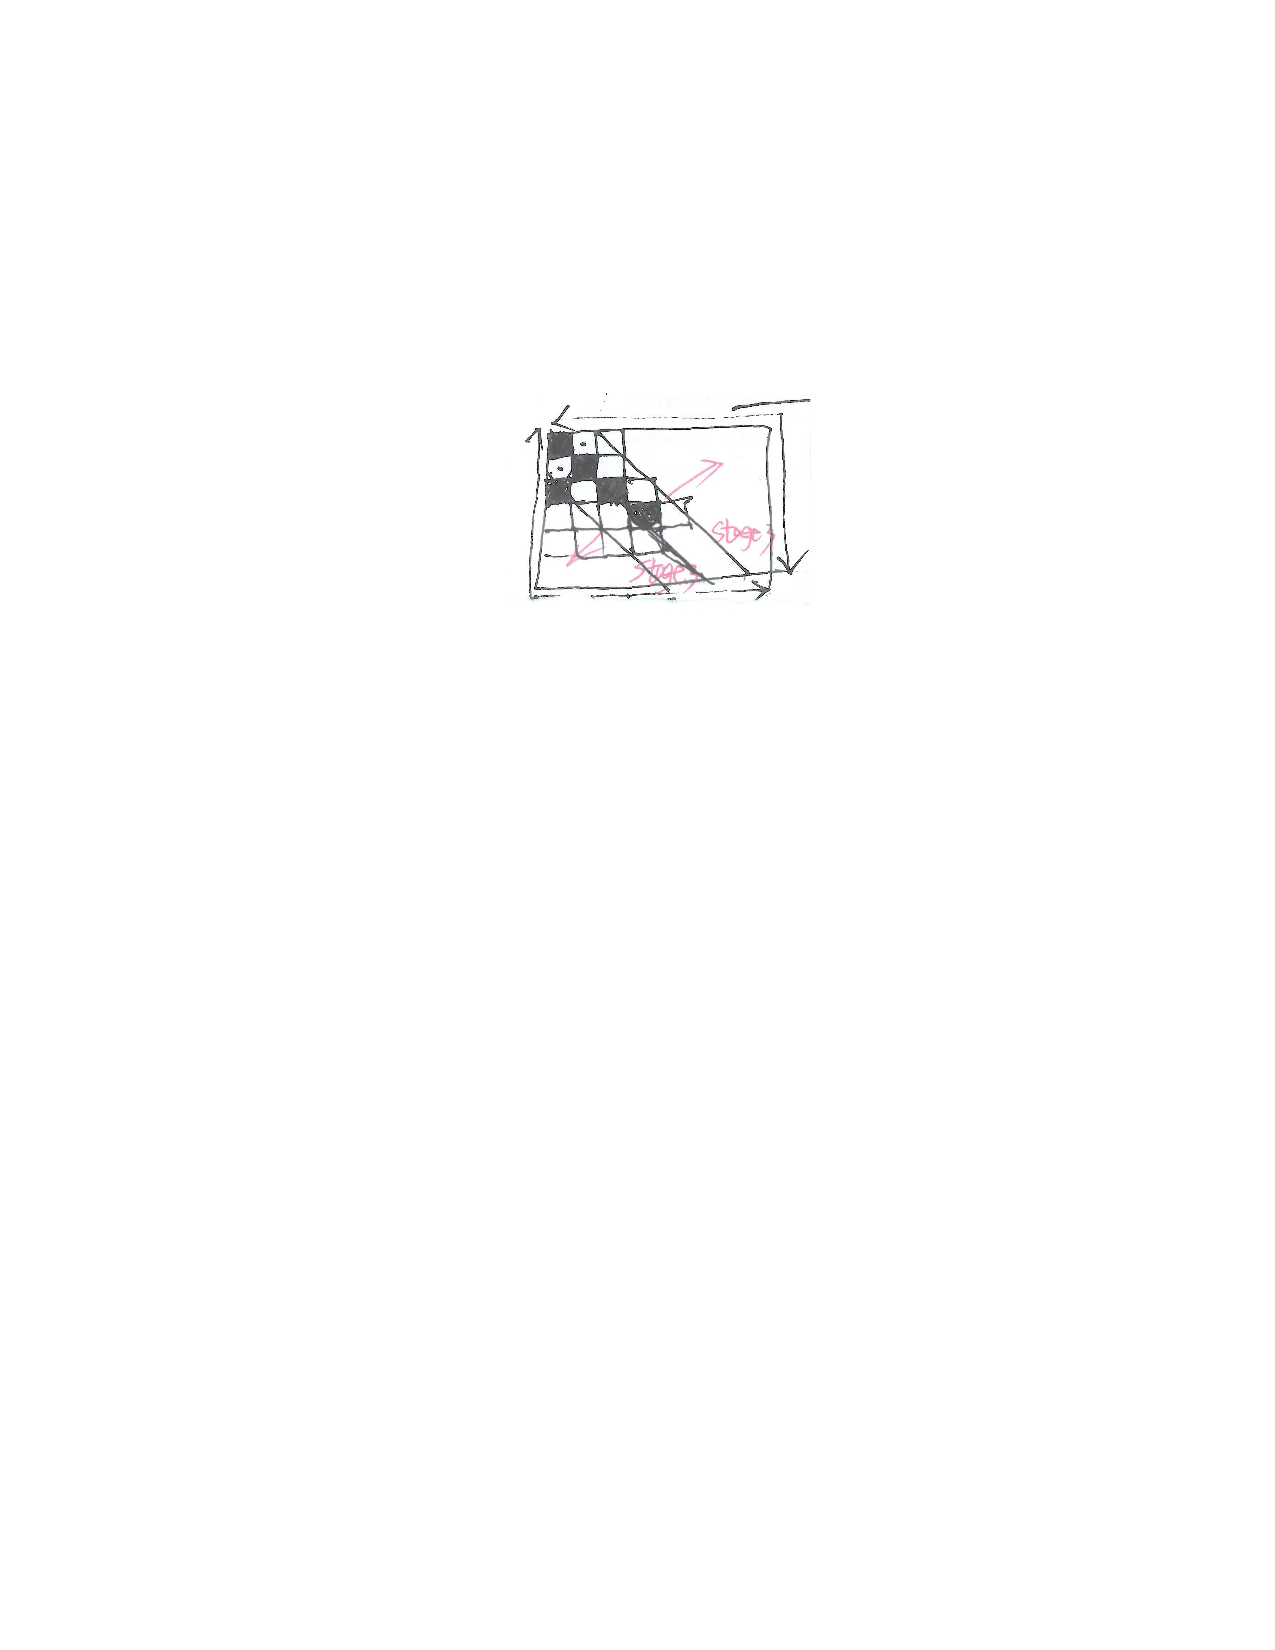
\includegraphics[scale=0.5]{figures/square.pdf}\\
  \caption{square}\label{square}
\end{figure}

\begin{figure}
  \centering
  % Requires \usepackage{graphicx}
  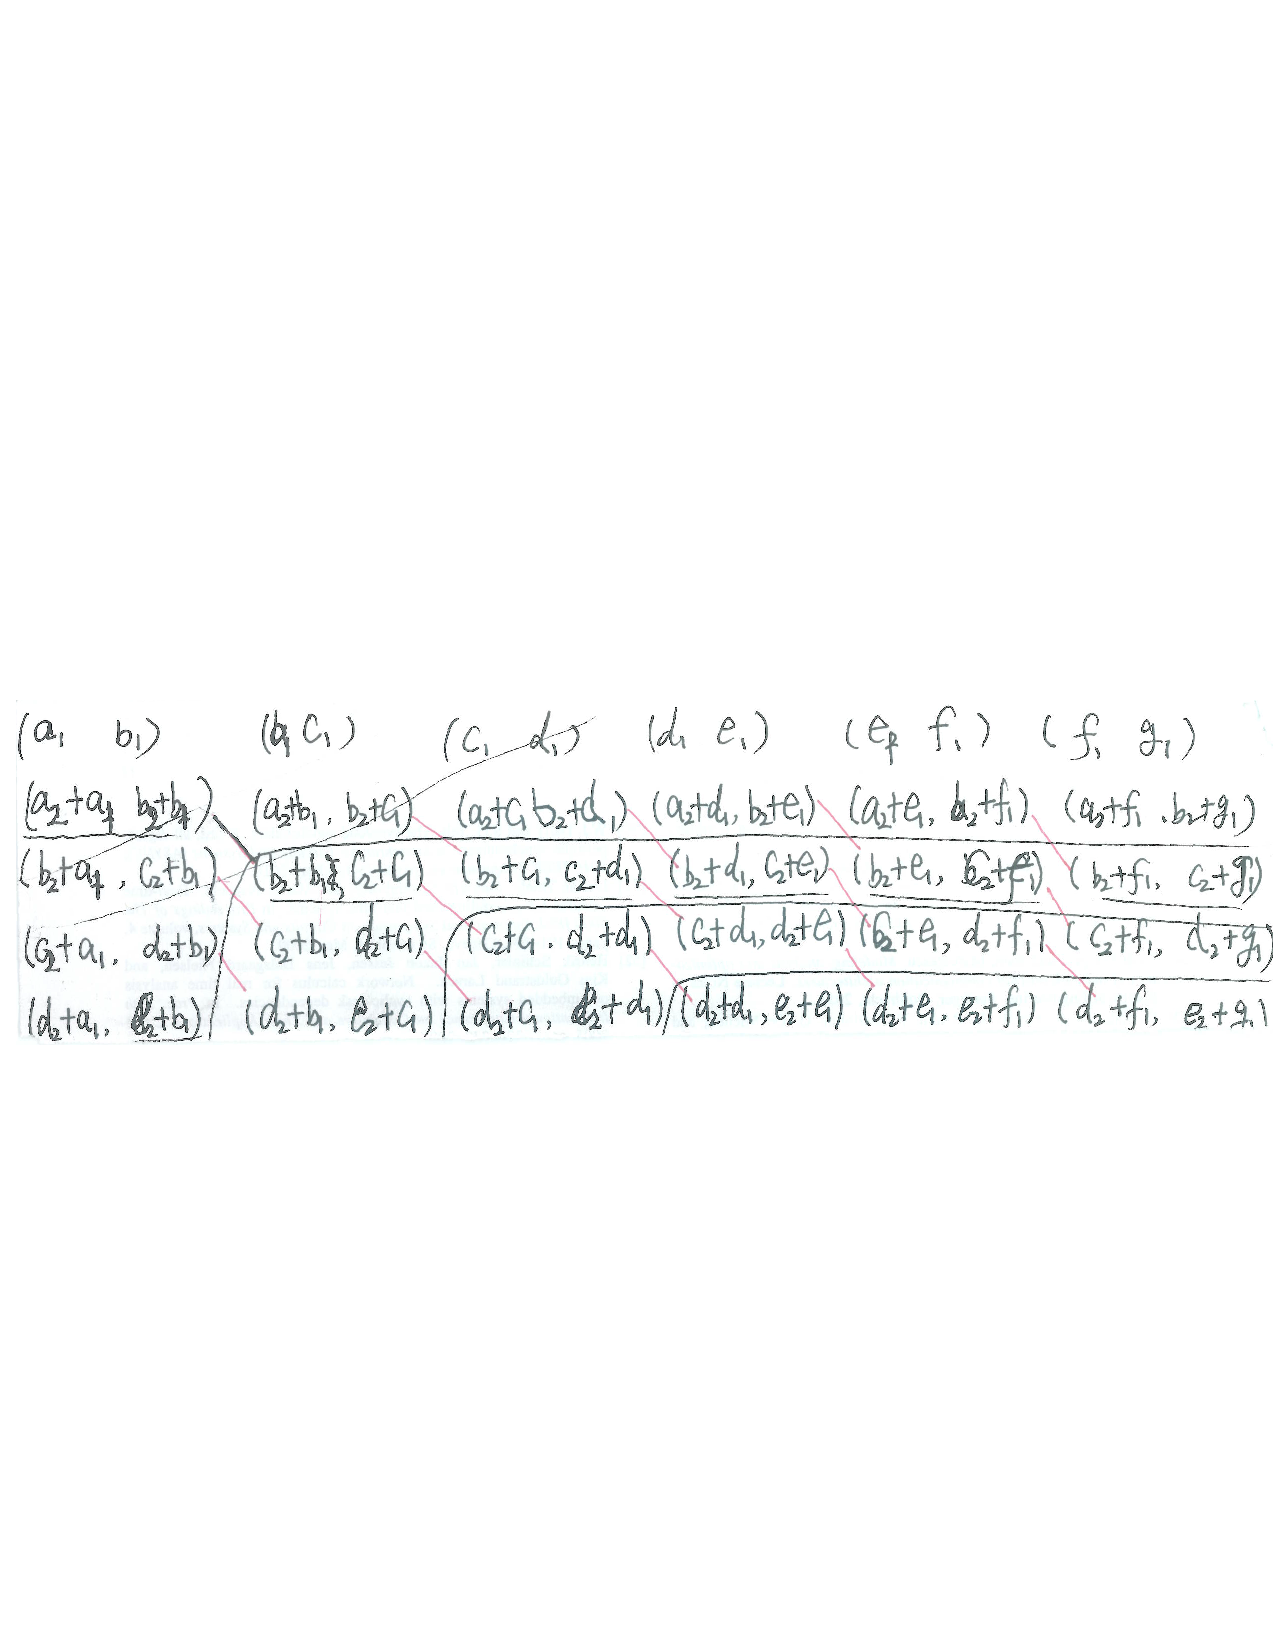
\includegraphics[scale=0.3]{figures/Matrix.pdf}\\
  \caption{matrix}\label{matrix}
\end{figure}

\subsection{实现基于OpenCl的并行算法}
1.OpenCL的简介
2.基于OpenCL实现的核函数

通过对问题的分析和研究,我们发现,该问题可以对应为对下凸包的计算。即点集中最左边的顶和最右边的点的连线以下的点集。在本应用场景中,对最左边的顶和最右边的点的计算非常容易,因为它就是对角线两个顶点上的值。

该算法在最快的情况下,只需要1次迭代就可以找到凸包(对应于阶梯函数的情况)。

\section{实验验证}\label{experiments}
1.实验平台
2.实验数据
3.实验结果

算法计算结果的加速比和正确性通过与已有的工具箱的比较得到。

\section{总结}
网络演算面向实用的重要一步就是数学模型的快速计算。

\bibliographystyle{unsrt}
\bibliography{Docear}

\end{document} 